% !TEX root = poster.tex
\node [mybox,anchor=north west, font=\fontsize{\fntszL}{\fntszL}\selectfont]
at (\bayesPos) (boxBayes){%
\begin{minipage}{\bxszB}

 \bigskip

\medskip
\centerline{
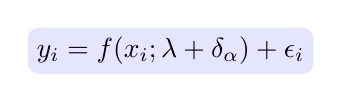
\begin{tikzpicture} \node [rounded corners,fill=blue!10] {
$y_i=f(x_i;\lambda+\delta_\alpha)+\epsilon_i$
};
\end{tikzpicture}
}

\bi
\item Given data $y_i$, perform \emph{simultaneous} estimation of \\$\tlam=(\lambda,\alpha)$, i.e. model parameters $\lambda$ and model-error parameters $\alpha$.
\item Bayes' theorem
\[
\overbrace{p(\tlam|y)}^{\textrm{Posterior}}= \frac{\overbrace{p(y|\tlam)}^{\textrm{Likelihood}} \overbrace{p(\tlam)}^{\textrm{Prior}}}{\underbrace{p(y)}_{\textrm{Evidence}}}
\]

\vspace*{2mm}

\item  To estimate the likelihood $L_y(\tlam)=p(y|\tlam)=p(y|\lambda,\alpha)$, one needs uncertainty propagation through  $\;f(x_i;\underbrace{\lambda+\delta_\alpha}_{\textrm{stochastic}})$
\vspace*{1mm}

%\item We employ Polynomial Chaos (PC) representation for $\delta_\alpha$.
\ei

\end{minipage}
};
\node[fancytitle, right=10pt, font=\fontsize{\fntszL}{\fntszL}\selectfont]
at (boxBayes.north west) {\bf Bayesian Estimation of Model Error};
